% Template for PLoS
% Version 3.5 March 2018
%
% % % % % % % % % % % % % % % % % % % % % %
%
% -- IMPORTANT NOTE
%
% This template contains comments intended
% to minimize problems and delays during our production
% process. Please follow the template instructions
% whenever possible.
%
% % % % % % % % % % % % % % % % % % % % % % %
%
% Once your paper is accepted for publication,
% PLEASE REMOVE ALL TRACKED CHANGES in this file
% and leave only the final text of your manuscript.
% PLOS recommends the use of latexdiff to track changes during review, as this will help to maintain a clean tex file.
% Visit https://www.ctan.org/pkg/latexdiff?lang=en for info or contact us at latex@plos.org.
%
%
% There are no restrictions on package use within the LaTeX files except that
% no packages listed in the template may be deleted.
%
% Please do not include colors or graphics in the text.
%
% The manuscript LaTeX source should be contained within a single file (do not use \input, \externaldocument, or similar commands).
%
% % % % % % % % % % % % % % % % % % % % % % %
%
% -- FIGURES AND TABLES
%
% Please include tables/figure captions directly after the paragraph where they are first cited in the text.
%
% DO NOT INCLUDE GRAPHICS IN YOUR MANUSCRIPT
% - Figures should be uploaded separately from your manuscript file.
% - Figures generated using LaTeX should be extracted and removed from the PDF before submission.
% - Figures containing multiple panels/subfigures must be combined into one image file before submission.
% For figure citations, please use "Fig" instead of "Figure".
% See http://journals.plos.org/plosone/s/figures for PLOS figure guidelines.
%
% Tables should be cell-based and may not contain:
% - spacing/line breaks within cells to alter layout or alignment
% - do not nest tabular environments (no tabular environments within tabular environments)
% - no graphics or colored text (cell background color/shading OK)
% See http://journals.plos.org/plosone/s/tables for table guidelines.
%
% For tables that exceed the width of the text column, use the adjustwidth environment as illustrated in the example table in text below.
%
% % % % % % % % % % % % % % % % % % % % % % % %
%
% -- EQUATIONS, MATH SYMBOLS, SUBSCRIPTS, AND SUPERSCRIPTS
%
% IMPORTANT
% Below are a few tips to help format your equations and other special characters according to our specifications. For more tips to help reduce the possibility of formatting errors during conversion, please see our LaTeX guidelines at http://journals.plos.org/plosone/s/latex
%
% For inline equations, please be sure to include all portions of an equation in the math environment.
%
% Do not include text that is not math in the math environment.
%
% Please add line breaks to long display equations when possible in order to fit size of the column.
%
% For inline equations, please do not include punctuation (commas, etc) within the math environment unless this is part of the equation.
%
% When adding superscript or subscripts outside of brackets/braces, please group using {}.
%
% Do not use \cal for caligraphic font.  Instead, use \mathcal{}
%
% % % % % % % % % % % % % % % % % % % % % % % %
%
% Please contact latex@plos.org with any questions.
%
% % % % % % % % % % % % % % % % % % % % % % % %

\documentclass[10pt,letterpaper]{article}
\usepackage[top=0.85in,left=2.75in,footskip=0.75in]{geometry}

% amsmath and amssymb packages, useful for mathematical formulas and symbols
\usepackage{amsmath,amssymb}

% Use adjustwidth environment to exceed column width (see example table in text)
\usepackage{changepage}

% Use Unicode characters when possible
\usepackage[utf8x]{inputenc}

% textcomp package and marvosym package for additional characters
\usepackage{textcomp,marvosym}

% cite package, to clean up citations in the main text. Do not remove.
% \usepackage{cite}

% Use nameref to cite supporting information files (see Supporting Information section for more info)
\usepackage{nameref,hyperref}

% line numbers
\usepackage[right]{lineno}

% ligatures disabled
\usepackage{microtype}
\DisableLigatures[f]{encoding = *, family = * }

% color can be used to apply background shading to table cells only
\usepackage[table]{xcolor}

% array package and thick rules for tables
\usepackage{array}

% create "+" rule type for thick vertical lines
\newcolumntype{+}{!{\vrule width 2pt}}

% create \thickcline for thick horizontal lines of variable length
\newlength\savedwidth
\newcommand\thickcline[1]{%
  \noalign{\global\savedwidth\arrayrulewidth\global\arrayrulewidth 2pt}%
  \cline{#1}%
  \noalign{\vskip\arrayrulewidth}%
  \noalign{\global\arrayrulewidth\savedwidth}%
}

% \thickhline command for thick horizontal lines that span the table
\newcommand\thickhline{\noalign{\global\savedwidth\arrayrulewidth\global\arrayrulewidth 2pt}%
\hline
\noalign{\global\arrayrulewidth\savedwidth}}


% Remove comment for double spacing
%\usepackage{setspace}
%\doublespacing

% Text layout
\raggedright
\setlength{\parindent}{0.5cm}
\textwidth 5.25in
\textheight 8.75in

% Bold the 'Figure #' in the caption and separate it from the title/caption with a period
% Captions will be left justified
\usepackage[aboveskip=1pt,labelfont=bf,labelsep=period,justification=raggedright,singlelinecheck=off]{caption}
\renewcommand{\figurename}{Fig}

% Use the PLoS provided BiBTeX style
% \bibliographystyle{plos2015}

% Remove brackets from numbering in List of References
\makeatletter
\renewcommand{\@biblabel}[1]{\quad#1.}
\makeatother



% Header and Footer with logo
\usepackage{lastpage,fancyhdr,graphicx}
\usepackage{epstopdf}
%\pagestyle{myheadings}
\pagestyle{fancy}
\fancyhf{}
%\setlength{\headheight}{27.023pt}
%\lhead{
\includegraphics[width=2.0in]{PLOS-submission.eps}}
\rfoot{\thepage/\pageref{LastPage}}
\renewcommand{\headrulewidth}{0pt}
\renewcommand{\footrule}{\hrule height 2pt \vspace{2mm}}
\fancyheadoffset[L]{2.25in}
\fancyfootoffset[L]{2.25in}
\lfoot{\today}

%% Include all macros below

\newcommand{\lorem}{{\bf LOREM}}
\newcommand{\ipsum}{{\bf IPSUM}}





\usepackage{forarray}
\usepackage{xstring}
\newcommand{\getIndex}[2]{
  \ForEach{,}{\IfEq{#1}{\thislevelitem}{\number\thislevelcount\ExitForEach}{}}{#2}
}

\setcounter{secnumdepth}{0}

\newcommand{\getAff}[1]{
  \getIndex{#1}{}
}

\providecommand{\tightlist}{%
  \setlength{\itemsep}{0pt}\setlength{\parskip}{0pt}}

\begin{document}
\vspace*{0.2in}

% Title must be 250 characters or less.
\begin{flushleft}
{\Large
\textbf\newline{Data collection of doctors recommended by the US immigration offices
using web scraping techniques in R.} % Please use "sentence case" for title and headings (capitalize only the first word in a title (or heading), the first word in a subtitle (or subheading), and any proper nouns).
}
\newline
% Insert author names, affiliations and corresponding author email (do not include titles, positions, or degrees).
\\
Rutendo Madziwo\textsuperscript{\getAff{Smith College}},
Maggie Szlosek\textsuperscript{\getAff{Smith College}},
Rachel LaFlamme\textsuperscript{\getAff{Smith College}}\\
\bigskip
\bigskip
\end{flushleft}
% Please keep the abstract below 300 words
\section*{Abstract}
Our client, ProPublica wants to know the doctors recommended by the US
government to green card applicants who have outstanding malpractice
suits against them. However, they do not know who these doctors are and
where they are located. Our focus is to collect information of all the
doctors on the US immigration website. This project aims to scrape data
from an interactive government website that has no endpoint urls using R
and Docker so as to give this data to our client.

% Please keep the Author Summary between 150 and 200 words
% Use first person. PLOS ONE authors please skip this step.
% Author Summary not valid for PLOS ONE submissions.

\linenumbers

% Use "Eq" instead of "Equation" for equation citations.
\section{Introduction}\label{introduction}

We worked under the direct instruction of ProPublica for their article
on medical malpractice among doctors recommended to green card
applicants. The question they were trying to answer with this research
was \emph{How many doctors recommended by the US government to green
card applicants have outstanding malpractice suits against them?} This
is the main question our research is attempting to help answer by
supplying them data to support their assumptions.

More specifically within this project, we are trying to answer \emph{Who
are the doctors being recommended to green card applicants, and how many
are there?}. As there is no reliable and searchable database released by
the government or any other entity that can be compared with a list of
doctors with malpractice suits against them, we will collect this data
and create this database for ProPublica for use in their article.

\section{Background}\label{background}

ProPublica is a news website that is focused on investigative journalism
that ``expose{[}s{]} abuses of power and betrayals of the public trust
by government, business, and other institutions, using the moral force
of investigative journalism to spur reform through the sustained
spotlighting of wrongdoing.'' {[}1{]} It was established in 2008 in New
York, NY, and continues to uphold this mission statement in a variety of
disciplines, including but not limited to politics, civil rights, and
education.

ProPublica plans on writing an upcoming article on doctors who have
malpractice claims against them, but are still being recommended by the
government to green card applicants. In order for an applicant to
receive a green card, they must have an appointment and full examination
with a state-sanctioned doctor. All of these recommended doctors can be
found on the government's \href{my.uscis.gov/findadoctor}{immigration
website}.

Because this examination is necessary for green card applicants and if
something goes wrong, the applicants are usually concerned that they may
not receive their green card if they report any cases of malpractice by
these doctors. ProPublica has collected testimonies of green card
applicants that have experienced instances that would constitute
malpractice, but did not report it to either the government or any other
entity in fear of not being able to immigrate, which means that these
doctors are still practicing and still being recommended by the
government for these examinations.

While these testimonies appear to be the main part of the upcoming
article, ProPublica would like to back their claims using data by
comparing doctors who are known to have malpractice suits filed against
them in the past with doctors who are recommended to green card
applicants via the government website. ProPublica currently has a list
of the doctors with malpractice violations, but there is no reliable
list of doctors approved by the goverment to give these examinations.

We were responsible for data collection of the names and contact
information of all of the doctors found on the
\href{my.uscis.gov/findadoctor}{website} and compilation of this data
into an easily understood file that could be compared with the
preexisting list of doctors with known malpractice suits. In order to do
this, we scraped the data found on this website.

This research is significant because allowing abusive doctors to work
does not only encourage them to not abide by the
\href{https://en.wikipedia.org/wiki/Hippocratic_Oath}{Hippocratic Oath}
risks the safety of immigrants while violating human rights. The
immigrants are in a vulnerable position because of their non-permanent
residential status, and thus could be taken advantage of. Additionally,
they may not be aware of some of the laws regarding professional
services in the US. This project will help expose the doctors and will
be a helpful aid in making sure that no future malpractices will occur.

We created a dataset based on the entries listed on the USCIS Find a
Doctor website. Each entry on the website contains the name of the
medical facility, name of the government-recommended doctor or doctors,
and the address and phone number of the facility. However, the search
bar on the website can only be used to search for doctors using US
zipcode or city name. Given that there are approximately 42,000 zipcodes
in the U.S. and no reliable dataset that contains all the current
zipcodes. The website is also structured in such a way that there are
only 10 entries per webpage; however, when the user clicks the next
button, they can see the doctors that are from a further radius than the
initially typed zipcode. They can click the next button to span an
approximately 500 mile radius before the website no longer provides a
`next' button.

For other websites, it is common to see that the search entry appears at
the end of the url which would allow each url to have a single
corresponding html page. On the other hand, the USCIS website contains
thousands of html pages housed under one url. The website has a static
url of https://my.uscis.gov/findadoctor regardless of the search entry
and this eliminates a plethora of traditional web-scraping methods.

We therefore looked for other methods for R to interact with the webpage
in order to bypass the non-changing url but still scrape the unique html
pages accurately and effectively.

\section{Methods}\label{methods}

As a starting point, we selected about 40 different zipcodes for
scraping our data based on our radius map. We then collected the
doctors' data using the package \texttt{rvest} for web-scraping,
\texttt{RSelenium} for web navigation and an external platform Docker
for virtual interaction with the web browser.

\begin{figure}
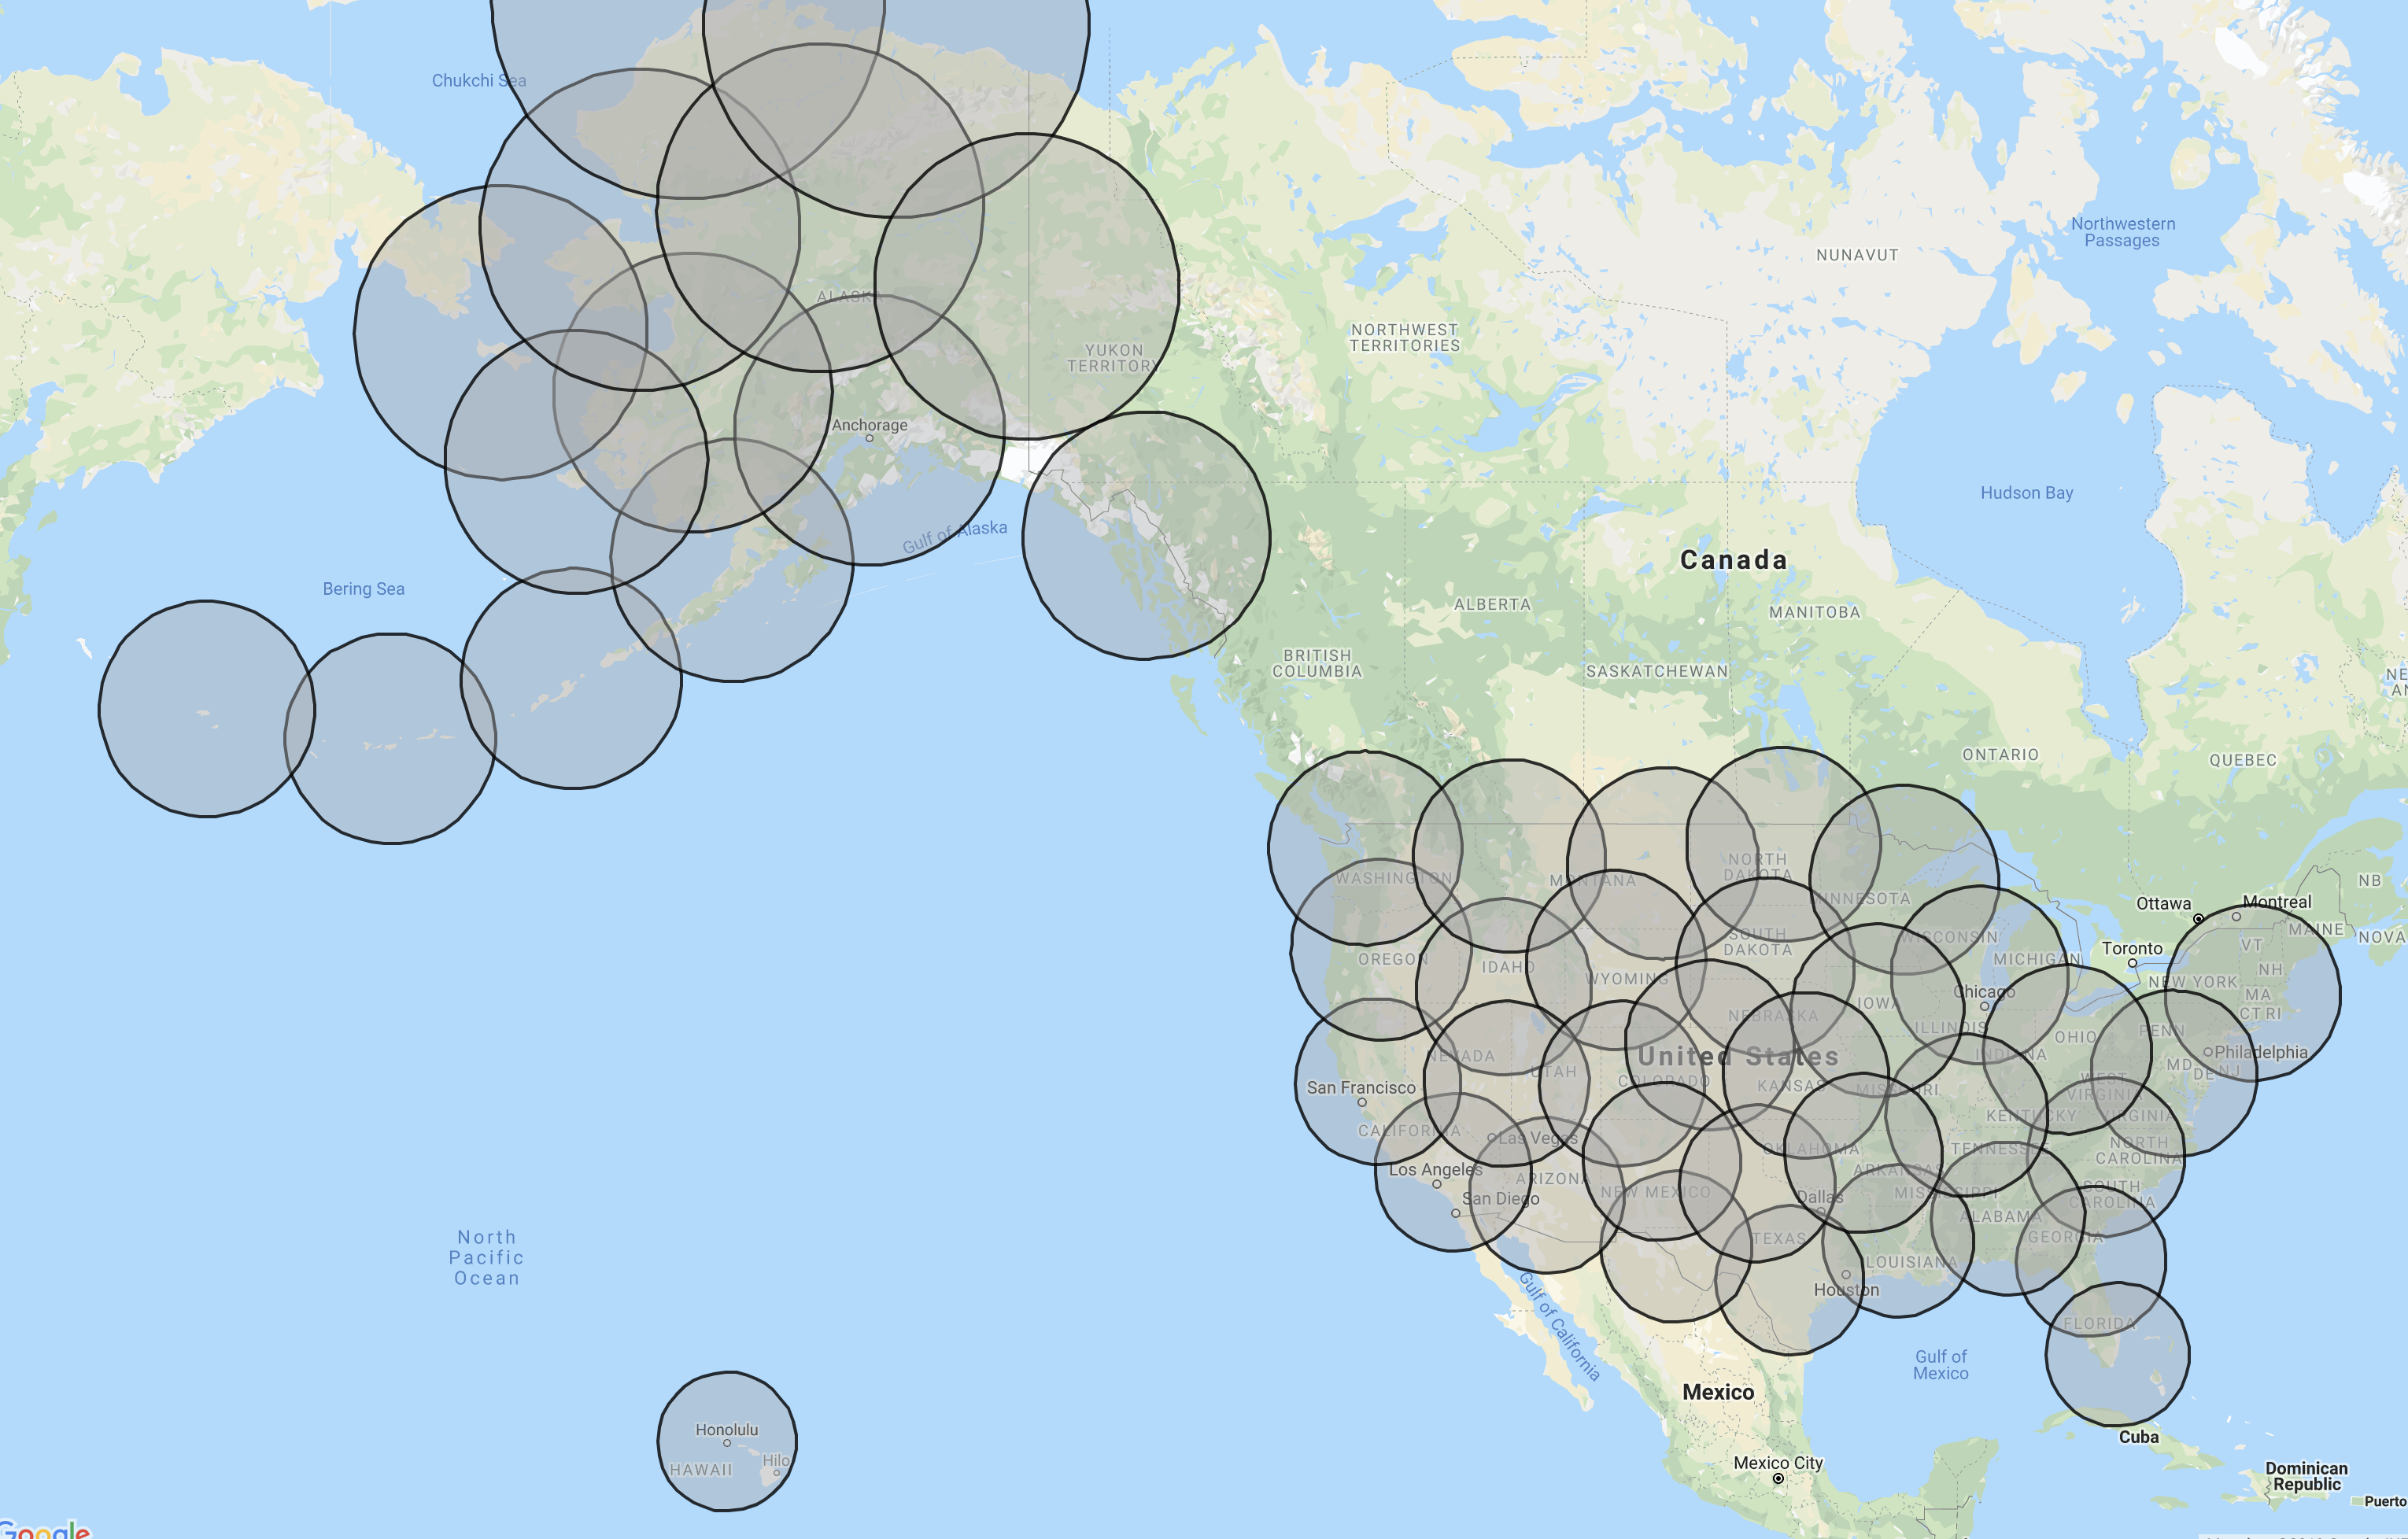
\includegraphics[width=1\linewidth]{RadiusMap} \caption{Radius Map}\label{fig:unnamed-chunk-1}
\end{figure}

\subsection{Tools used}\label{tools-used}

\subsection{\texorpdfstring{\texttt{Docker}}{Docker}}\label{docker}

Docker is a platform to develop, deploy, and run applications inside
containers{[}2{]}. We were able to virtually interact with the USCIS
website by connecting to a port in Docker and opening Chrome and this
enabled us to control and see what was happening on the website at a
given time. Initially, Docker was installed before installing and
loading the necessary R Packages. The command
\texttt{docker\ run\ -d\ -p\ 4445:4444\ selenium/standalone-chrome} was
then run in the R Terminal as a shell command after we had installed our
packages. This command sets up the virtual Chrome container to enable
interaction with the Chrome web browser. In order to check if Docker is
running, one can type in \texttt{docker\ ps}. We eventually open the
browser using RSelenium commands before scraping our data.

\begin{figure}
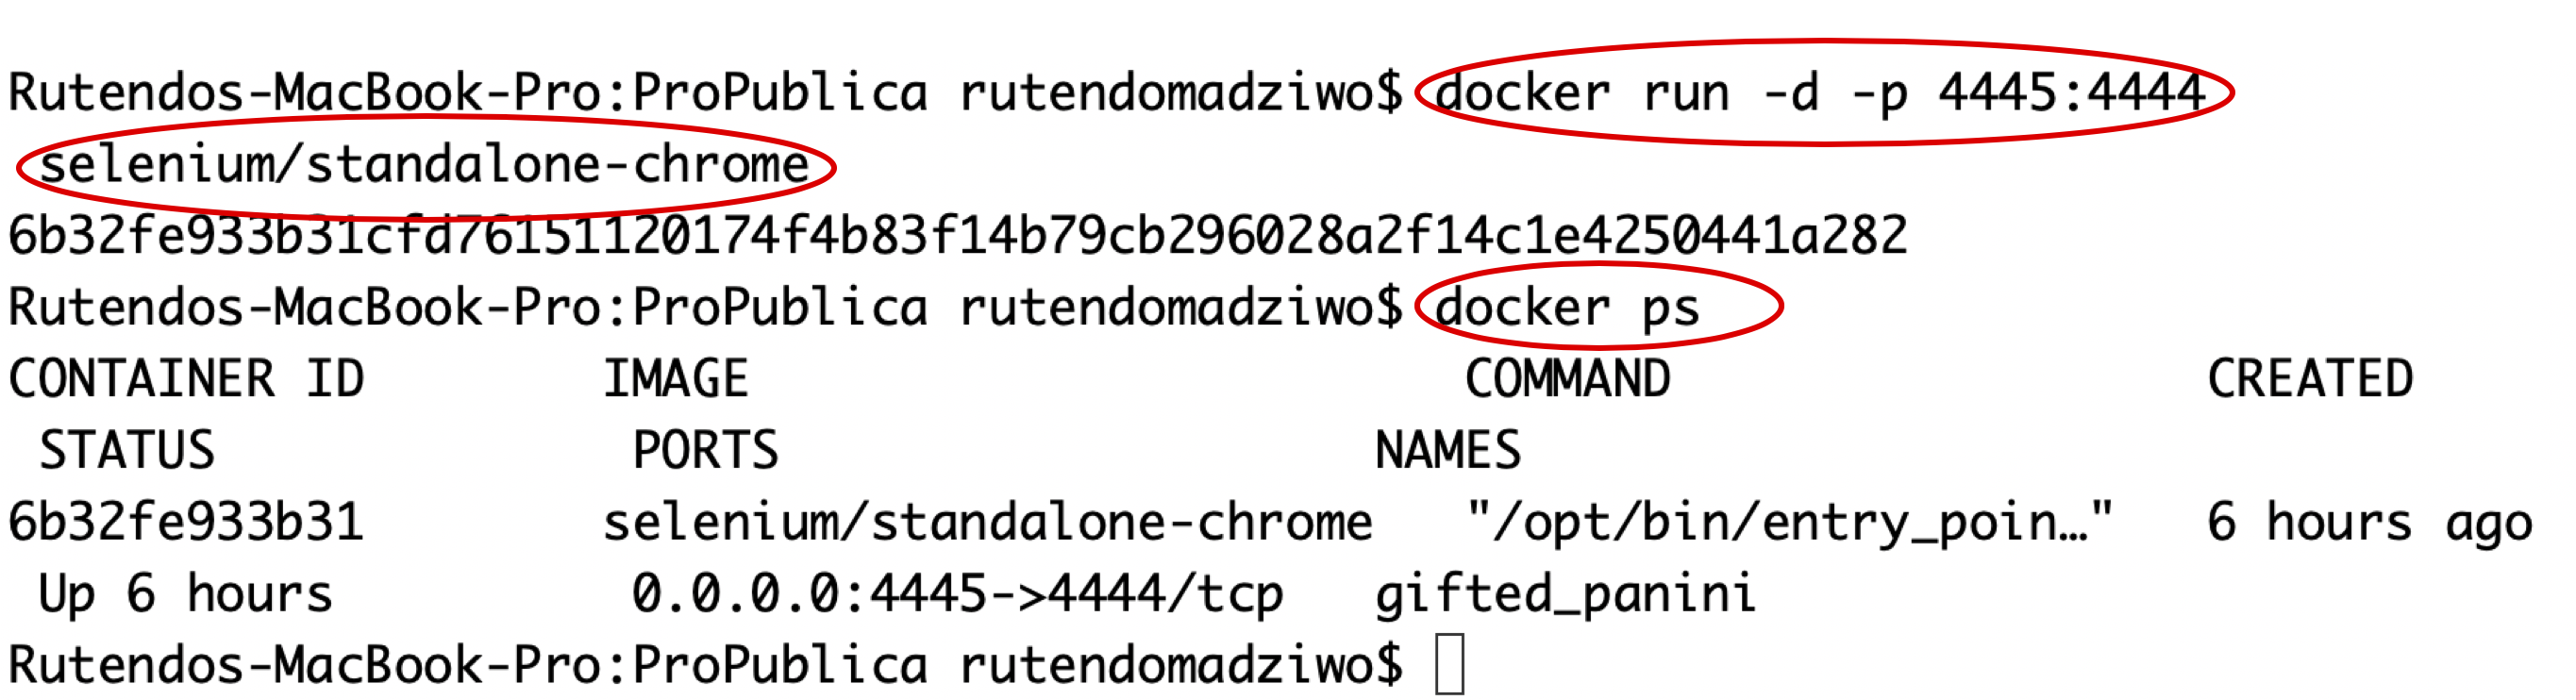
\includegraphics[width=1\linewidth]{docker_start} \caption{Docker Setup}\label{fig:unnamed-chunk-2}
\end{figure}

\subsection{\texorpdfstring{\texttt{RSelenium}}{RSelenium}}\label{rselenium}

RSelenium is a package in R which helps one connect to a Selenium server
{[}3{]}. This server in turn connects to the Chrome web browser and
hence allowed us to automate our webscraping experience. RSelenium is
responsible not only for opening and closing the browser, but it allowed
us to virtually navigate the web page and automatically control the
scraping. This was especially useful as our website had no endpoint urls
and hence could not rely on more traditional web scraping methods. In
addition, it made the process of scraping the data faster as one can
simply allow the code to run, programatically click the Next button on
the web page and hence scrape multiple pages without needing to manually
click the specific website.

\begin{figure}
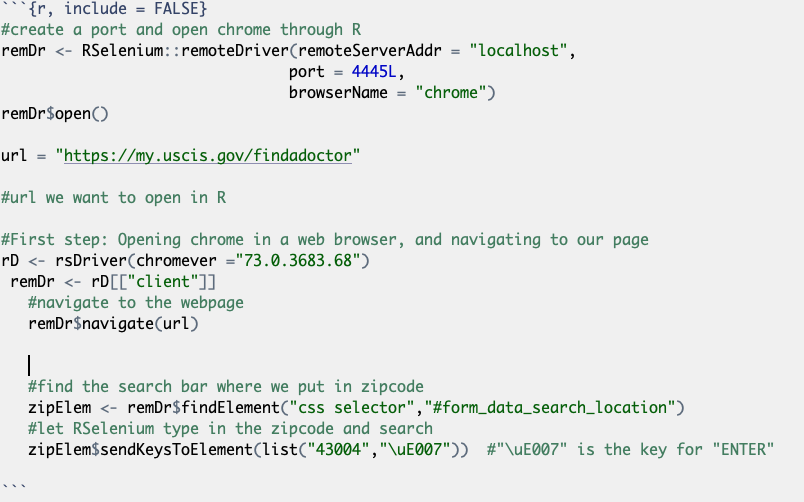
\includegraphics[width=1\linewidth]{docker_selenium} \caption{Illustration of Doker and RSelenium Interaction}\label{fig:unnamed-chunk-3}
\end{figure}

\subsection{\texorpdfstring{\texttt{rvest}}{rvest}}\label{rvest}

While RSelenium was responsible for most of the web manouvering, the
package we used for scraping the data from each of the pages was
\texttt{rvest} {[}4{]}. This package makes harvesting data from a
website easy as it can find specific html nodes, and their children. It
also allows one to use both XPaths and CSS selectors so though we
eventually stuck to using basic elements, we were not limited to one
option. As a side note, we chose to use CSS selectors for web navigation
with the RSelenium package.

\section{Data Collection}\label{data-collection}

We created a function to scrape this data and took advantage of the
purrr package in R to map all our scraped elements together. This
function was able to scrape all the exception datapoints that contained
different or missing nodes from our standard entries with one doctor per
medical facility such as multiple approvied doctors working in one
facility and entries with no phone numbers listed. To clean up our data,
\texttt{dplyr} and \texttt{tidyverse} were used for text-processing the
such that zipcodes, states, and cities, were in separate columns from
the rest of the address in the resulting doctors' dataset
{[}5{]}{[}6{]}.

The final code written to collect the doctors' information allows a user
to input one zipcode at a time in order to scrape data. Once that
zipcode is entered, the doctors and facilities on that web page are
harvested using \texttt{rvest} before moving on to the next page.
Clicking to the next page has been automated using \texttt{RSelenium}
and a for loop was implemented in our code such that for a certain
number of times, the website's \texttt{Next} button is clicked, moves on
to the next page, scrapes that page and so on. The website itself has
been written in such a way that an actual user can keep clicking to find
the nearest doctors within a 500 miles radius. As such, we have also
manually entered different zipcodes in different parts of the USA so as
to capture all the doctors in the country and create different datasets.

\begin{figure}
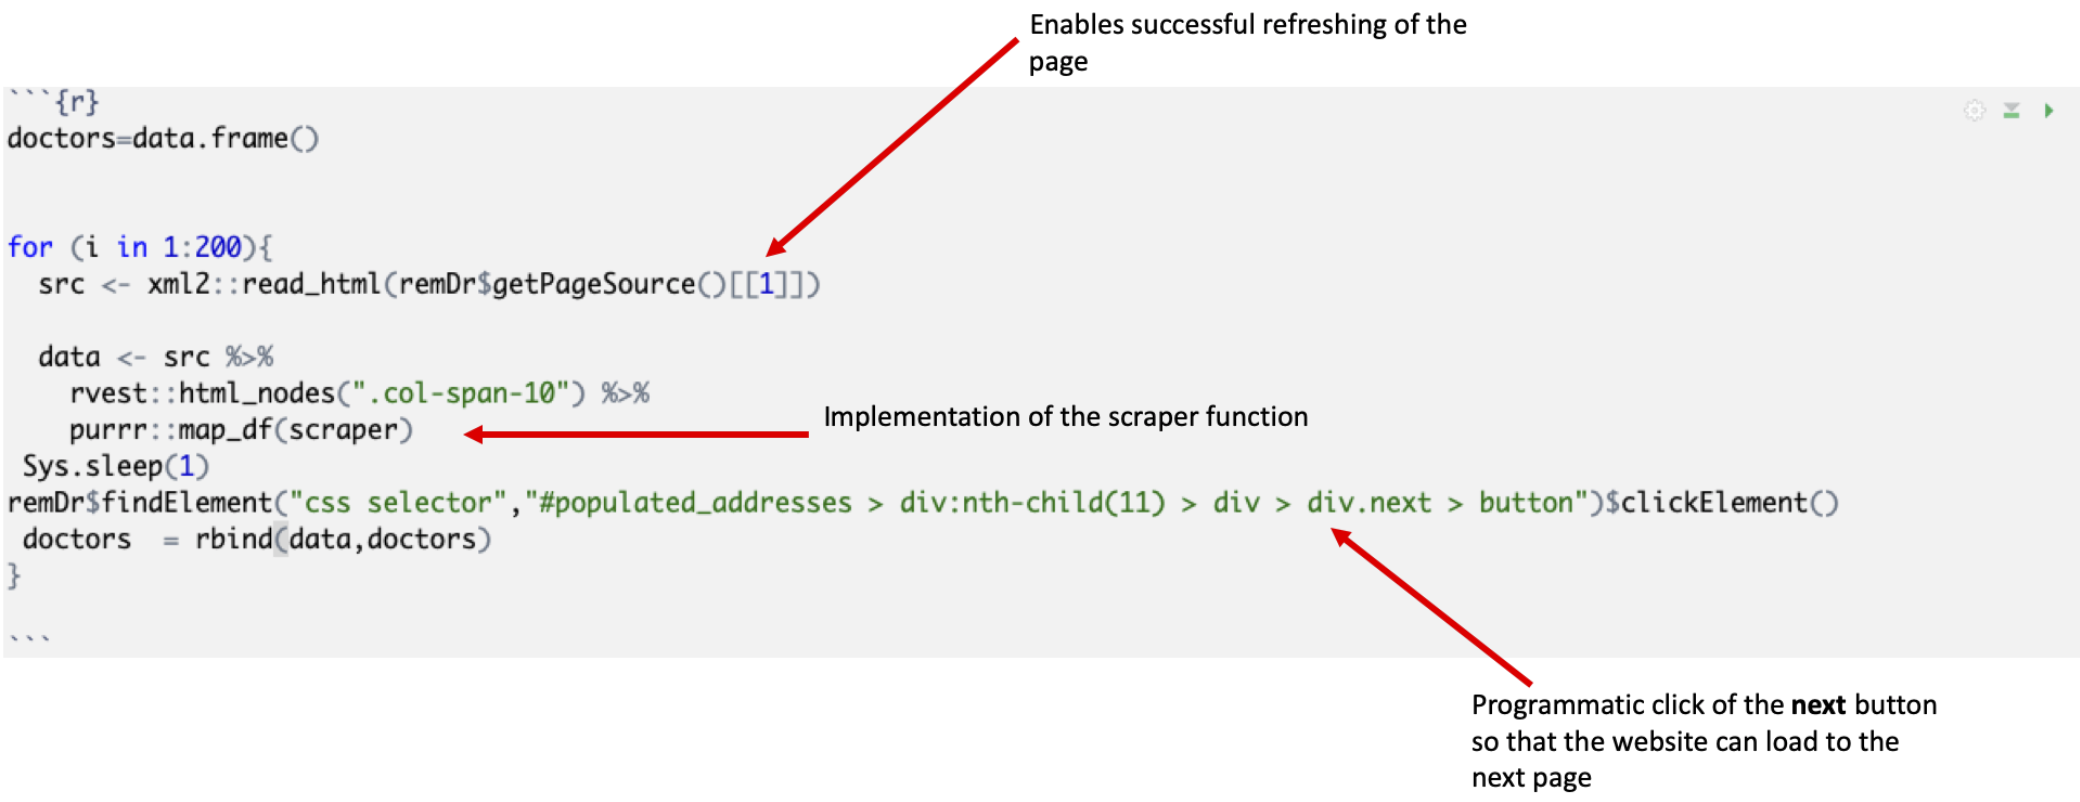
\includegraphics[width=1\linewidth]{final_scrape} \caption{Illustration of final scraping method}\label{fig:unnamed-chunk-4}
\end{figure}

\section{Results}\label{results}

At this time, we have been able to build an algorithm that accurately
scrapes the website of all doctors within a 500-mile radius of a
starting zip code, at which time the website no longer has a `next'
button. Then the code must run separately from a different origin point
in order to find more doctors recommended by the website. At this point,
we have run the code from three different locations including
Northampton, Miami, and a remote location in Arizona and are still
scraping the other locations. ProPublica asked for a dataset that is
organized by the following variables: name, address, city, state,
zipcode, and phone number which is representative of all the
government-approved doctors in the entirety of the United States at the
time the website was scraped and have created this dataset. Since our
dataset contains all categorical and string entries, minimal statistical
work can be done aside from some summary statistics of the number of
doctors scraped per zipcode, state, etc.(Results to follow)

\section{Discussion}\label{discussion}

This data is useful because, based on information we received from our
client, the scraping of this data from this website had not been
reliably undertaken until now. This could be an important resource not
just to understanding how prevalent medical malpractice is among this
group of doctors immigrants are required to see, but also to find other
trends possible within this group. In addition, we know that this will
potentially help immigrants who are being taken advantage of by the
current system, in which no protections are put in place against
malpractice violations.

\section{Limitations}\label{limitations}

There were a number of limitations we have with the current research and
our product. Because of the method in which the website is set up, in
order to get a full list of all of the doctors in the country, the code
must be run multiple times from multiple origin points. If one needs
just one region, this code will work much more quickly, but will not
grant the user a full look at all of the doctors that are recommended by
uscis.gov. This means that, even though we determined that this was the
best example of code we could use, because of the format of the website,
it still takes a long time to run and must run multiple times. While we
hope to give a complete list to ProPublica of all doctors recommended,
if they wish to check or if someone else wishes to replicate our work,
the process for gathering data is relatively tedious. In addition, this
code was written specifically for this particular website, meaning that
it likely could not scrape data from a similar or even similar formatted
website, as it is largely based on the individual HTML coding of
uscis.gov. This makes the overall impact of this code on its own
relatively small.

In addition, this data was gathered specifically for the use of
ProPublica, meaning that we may not be able to spread this data without
their express permission. This puts limits on the usefulness of our
code, as the data could be used for other projects and transformed if
other outlets see fit, particularly because this data has never been
gathered before. However, because of ProPublica's role, we may not be
able to share this information.

Another potential problem is that we do not know exactly how ProPublica
plans to use this data set. While we understand the underlying goal, we
have not seen the list of doctors that our dataset will be compared to
and so we do not know whether or not the data will be used responsibly
and ethically. While we understand ProPublica's mission and stand by it,
and trust that our data will help rather than harm people, it is still a
concern that is currently on our minds.

This dataset has the potential to help with many things, in addition to
its intended purpose of contributing to this article on green card
applicants and medical malpractice, authored by ProPublica. In addition,
it could be used to compare doctors being recommended by the government
to, for example, general sexual assault charges or other crimes, or just
having a greater understanding of the types of medical doctors who are
being recommended to immigrants.

\section*{References}\label{references}
\addcontentsline{toc}{section}{References}

\hypertarget{refs}{}
\hypertarget{ref-ProPublica}{}
1. ProPublica the mission. \url{https://www.propublica.org/about/};

\hypertarget{ref-Docker}{}
2. Docker docker home page. \url{https://www.docker.com};

\hypertarget{ref-RSelenium}{}
3. RSelenium r bindings for selenium 2.0 remote webdriver.
\url{http://ropensci.github.io/RSelenium/};

\hypertarget{ref-rvest}{}
4. rvest easily harvest. \url{http://rvest.tidyverse.org};

\hypertarget{ref-dplyr}{}
5. dplyr a grammar of data manipulation.
\url{https://dplyr.tidyverse.org};

\hypertarget{ref-tidyverse}{}
6. tidyverse tidyverse. \url{https://www.tidyverse.org};

\nolinenumbers


\end{document}

